\begin{frame}{Failure Analysis Overview}
\begin{itemize}
    \item Analysis based on runtime logs and hardware monitor data from Kalos (32,500 tasks) and Seren (675 tasks)
    \item Focus on pretraining and inference tasks
    \item Goal: insights for fault-tolerance in LLMs
\end{itemize}
\end{frame}


\begin{frame}{Failure Categories}
\begin{itemize}
    \item \textbf{Infrastructure:} NVLink, CUDA, Node, ECC, Network; high GPU usage and long recovery
    \item \textbf{Framework:} RuntimeError, ValueError, AttributeError; often config related
    \item \textbf{Script:} Programming/user errors; majority of failures
\end{itemize}
\end{frame}


\begin{frame}{Key Observations}
\begin{itemize}
    \item Infrastructure failures consume \textgreater 82\% GPU resources, only 11\% of job count
    \item High GPU temperatures in Kalos can cause NVLinkError/ECCError
    \item Auxiliary services (logging, monitoring) can trigger Connection/Network errors
    \item Evaluation jobs rarely fail (\~6.7\%)
\end{itemize}
\end{frame}


\begin{frame}{Failure Statistics}
\begin{center}
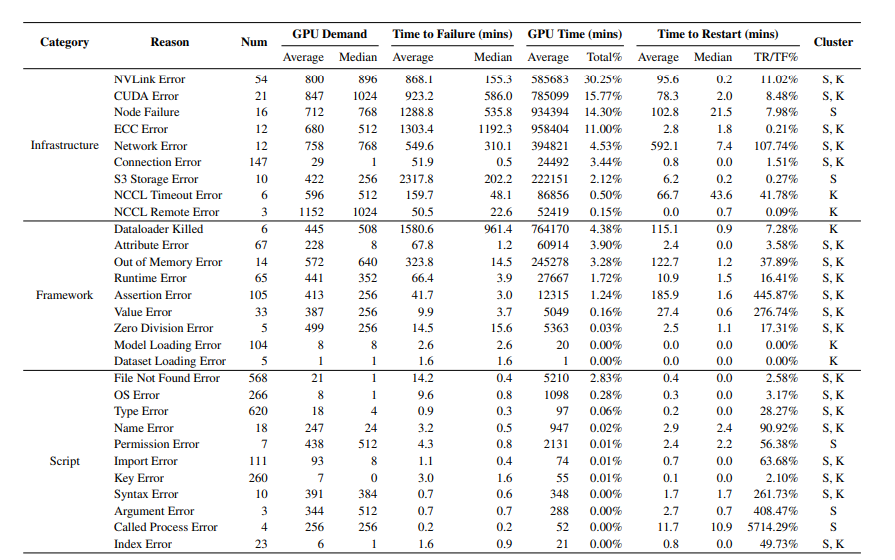
\includegraphics[width=0.9\textwidth,height=0.7\textheight,keepaspectratio]{figures/Failure Statistics.png}
\end{center}
\end{frame}


\begin{frame}{Failure Recovery}
\begin{itemize}
    \item Restart scenarios:
    \begin{enumerate}
        \item Job error occurs
        \item Loss spike or abnormal training metrics
        \item Training process stuck
    \end{enumerate}
    \item Jobs revert to last checkpoint on restart
    \item Manual recovery needed due to lack of automatic support
    \item Framework improvements reduced losses in later models (123B)
\end{itemize}
\end{frame}